
%%%%%%%%%%%%%%%%%%%%%%% file typeinst.tex %%%%%%%%%%%%%%%%%%%%%%%%%
%
% This is the LaTeX source for the instructions to authors using
% the LaTeX document class 'llncs.cls' for contributions to
% the Lecture Notes in Computer Sciences series.
% http://www.springer.com/lncs       Springer Heidelberg 2006/05/04
%
% It may be used as a template for your own input - copy it
% to a new file with a new name and use it as the basis
% for your article.
%
% NB: the document class 'llncs' has its own and detailed documentation, see
% ftp://ftp.springer.de/data/pubftp/pub/tex/latex/llncs/latex2e/llncsdoc.pdf
%
%%%%%%%%%%%%%%%%%%%%%%%%%%%%%%%%%%%%%%%%%%%%%%%%%%%%%%%%%%%%%%%%%%%


\documentclass[runningheads,a4paper]{llncs}

\usepackage{amssymb}
\setcounter{tocdepth}{3}
\usepackage{graphicx}
%\usepackage{hyphenat} see
%http://www.ctan.org/tex-archive/macros/latex/contrib/hyphenat - would
%be good to enable this to prevent hyphenation of OWL MS statements.
%Or find alternative

\usepackage{url}
%\urldef{\mailsa}\path|davidos@ebi.ac.uk|

\newcommand{\keywords}[1]{\par\addvspace\baselineskip
\noindent\keywordname\enspace\ignorespaces#1}

\begin{document}

\mainmatter  % start of an individual contribution

% first the title is needed
\title{Virtual Fly Brain - Using OWL to support the mapping and
  genetic dissection of the \textit{Drosophila} brain.}

% a short form should be given in case it is too long for the running head
\titlerunning{Virtual Fly Brain - using OWL to support Drosophila neurobiology}

% the name(s) of the author(s) follow(s) next
%
% NB: Chinese authors should write their first names(s) in front of
% their surnames. This ensures that the names appear correctly in
% the running heads and the author index.
%
\author{David Osumi-Sutherland$^1$, Marta Costa$^2$, Gregory S.X.E. Jefferis$^3$}

%
\authorrunning{Virtual Fly Brain - using OWL to support Drosophila neurobiology}
% (feature abused for this document to repeat the title also on left hand pages)

% the affiliations are given next; don't give your e-mail address
% unless you accept that it will be published
\institute{European Bioinformatics Institute, Wellcome Trust Genome
  Campus, Hinxton, Cams, UK}
% \mailsa\\  % This needs to be fixed!

%
% NB: a more complex sample for affiliations and the mapping to the
% corresponding authors can be found in the file "llncs.dem"
% (search for the string "\mainmatter" where a contribution starts).
% "llncs.dem" accompanies the document class "llncs.cls".
%

\toctitle{}
\tocauthor{}
\maketitle


\begin{abstract}
A massive effort is underway to map the struture of the \textit{Drosophila}
nervous system and to genetically dissect its function. Virtual Fly
Brain (VFB; http://www.virtualflybrain.org) is a popular, OWL-based resource
providing neuroinformatics support for this work.  Here we present
details of the current use of OWL on VFB  - underlying tools for
searching and querying across curated information from the literature
in combination with information mined from bulk data sets.

In order to keep reasoning fast and scalable, we have, up to now, restricted
expressiveness to the EL profile of OWL and used the ELK reasoner. As a result,
we have been unable to provide queries involving negation, despite
there being cases where there is clear
user demand and sufficient information to support these
queries. Recent developments in reasoning technology may
make these queries practical. We present ontology design patterns to
support the queries with negation that our users want.

\keywords{OWL, neurobiology, neuron, DL reasoning, negation, closure
  axioms, ontology design pattern}
\end{abstract}

\section{Introduction}


\subsection{Mapping and genetically dissecting the \textit{Drosophila}
  nervous system}


A massive effort is underway to map the neural circuitry of the
\textit{Drosophila} nervous system and to genetically dissect its
function. New microscopy and image analysis techniques are
facilitating the collection and integration of the massive 3D image
data sets required to map the structure and connectivity of the
nervous system down to the single neuron level [REFS]. New genetic % refs from grant
techniques allow researchers to precisely target elements of the
neural circuitry to inhibit or activate it in order assess the effects
of nervous system function and behavior [REFS]. The scale of this % refs from grant
effort, and the huge volumes of data involved, mean that its success
depends on suitable informatics support. Virtual Fly Brain (VFB)
\cite{pmid22180411,pmid22402613} is an OWL-based, open source
resource dedicated to this role. Usage is growing rapidly among the community
it serves.  The site currently gets 15-20,000 page views per month.

The adult \textit{Drosophila} nervous system contains an estimated
200,000 neurons [REF?].  These can be grouped into classes that share
similar location, morphology and lineage.  The number of such classes
is likely to be at least an order of magnitude smaller than the number
of neurons [REF - PC Rubin?].  Mapping the neural circuitry of \textit{Drosophila}
requires ways to track the classification of these neurons and their
properties, including their relationships to each other and to the
gross anatomy of the nervous system, musculature, sense organs and
neuro-endocrine system.  This work requires synthesis of many of
qualitative assertions from the literature and its integration with
information from bulk data sources, much of it quantitative.  OWL
is an ideal technology for building and maintaining these queryable
classifications. There will always be a need for direct mathematical
access to quantitative data.  But if suitable cutoffs can be
chosen to make qualitative assertions from quantitative data, OWL
provides a means to integrate qualitative and quantitative data into a
queryable whole.

Modulating the activity of specific neuron classes requires finding
reagents whose expression sufficiently specific. Finding such reagents
frequently requires mining 3D image data of expression patterns.
Integrating the phenotypic results of modulating neuronal activity
into the bigger picture of nervous system function requires ways to
keep track of the phenotypes associated with modulating the neuronal
activity of connected neurons.  Annotation with OWL ontology terms -
either semi-formalised in a database or fully formalised in an OWL
knowledgeBase provides a means of storing this information in
queryable form.

\subsection{The Drosophila anatomy ontology}

Virtual Fly Brain is built around the \textit{Drosophila} anatomy
ontology (DAO, Costa et al., 2013), an OWL ontology of
\textit{Drosophila} anatomy, over 45\% of which (3875/8576 classes) is
devoted to representing neuroanatomy. The DAO is largely manually
curated from the literature and includes a large textual component in
the form of referenced synonym lists and definitions/descriptions -
making it searchable by and accessible to biologists.  These are used
to drive auto-suggestion based searching on VFB and to populate term
information pages for specific neuron classes and nervous system
regions. The DAO is also richly formalised, using 44 object properties
in \textgreater 17000 Subclassing axioms and \textgreater 2000
Equivalent Class axioms.  This axiomatisation infers almost 50\% of
\textgreater 10,000 classifications and allows a rich variety of
biologically interesting queries.

\subsection{Annotation queries}

One major usage of VFB is as a means to query for expression of genes,
transgenes and phenotypes in specified anatomical classes.  These
queries use information curated from the literature and bulk data sets
by VFB and FlyBase curators using an semi-formalised tagging
system. All queries of these annotations start with a query for
subclasses, parts and overlapping cells.  The resulting list is then
used to query the FlyBase SQL database of annotations.  10's of
thousands of annotations are available from these queries.

% \subsection{other ontologies in VFB}

% % Need to decide whether to keep this thread
% The DAO has many axioms referencing Gene Ontology biological process
% classes via a \textbf{capable\_of} object property as a means of
% recording function in behaviour, sensory perception and
% neurophysiological processes.

% % Phenotype ontology


\section{OWL queries and design patterns for neuroanatomy}

The DAO uses an integrated set of relations and design patterns to
classify neurons according to their location, connectivity, lineage
and function \cite{pmid22180411,pmid22402613}.  The neuronal
connectivity relations, along with some basic mereological reasoning,
drive the query system on VFB (see figure
\ref{fig:Query_menus_DL_images}). VFB takes advantage of term
classification in the DAO to serve only queries that are
appropriate to the term displayed. So, for example, the queries
available for neurons are different to those available for brain regions.

The typical mereological relationship between a neuron and gross
neuroanatomy is overlap:  most neurons have parts in many
parts of the brain.  In an insect brain, each neuron has a cell body
(soma) in the cortex and has long, branching projections that extend
to multiple brain regions.  Many projections bundle (fasciculate)
together to form tracts.  On exiting a tract, the projection enters a
region called neuropil where it typically branches extensively and
connects to other neuron projections via synapses.

The \textit{Drosophila} brain contains many neuron classes that can be
defined via some combination of: soma location, tracts fasciculated
with; neuropils in which they form input or output synaptic
connections with other neurons; neuron classes synapsed with; the
developmental origin of the neuron.  The DAO takes advantage of this
to automate classification of neurons based on these properties via
EquivalentClass expressions.

Central to the basic mereological reasoning on VFB is an
\textbf{overlaps} relation defined using \textbf{part\_of} and its
inverse \textbf{has\_part}

\begin{quote}
X \textbf{overlaps} Y iff: \textit{exists some} Z \textit{and}
X \textbf{part\_of} Z \textit{and} Y \textbf{has\_part}
Z\footnote{\textbf{part\_of} and \textbf{has\_part} are both
  transitive and reflexive; \textbf{part\_of} \textit{inverseOf}
  \textbf{has\_part}}

\textbf{part\_of} \textit{subPropertyOf}
  \textbf{overlaps}

\textbf{has\_part} \textit{subPropertyOf} \textbf{overlaps}

\textbf{has\_part} \textit{o} \textbf{part\_of} \textit{subPropertyOf}
\textbf{overlaps}

\textbf{overlaps} \textit{o} \textbf{part\_of} \textit{subPropertyOf} \textbf{overlaps}

\textbf{has\_part} \textit{o} \textbf{overlaps} \textit{subPropertyOf}
\textbf{overlaps}\end{quote}

The property chains allow inference over partonomy.  This is central
to the function of the query system on VFB - allowing queries for
overlap from any level of granularity in the partonomy.

Typically, \textbf{overlaps} is too abstract to be directly useful in
class restrictions. Instead we use a range of subproperties of
\textbf{overlaps} that record something useful about the nature of the
overlap, such as which tract(s) a neuron fasciculates with and which
neuropils it form synapses in.  Like \textbf{overlaps}, relations
recording synaptic terminal location also propagate over partonomy via
property chains, allowing queries from any level of the partonomy.
For example:

\begin{quote}
\textbf{has\_synaptic\_terminal\_in} \textit{o} \textbf{part\_of} \textit{subPropertyOf}
\textbf{has\_synaptic\_terminal\_in}

\textbf{has\_part} \textit{o} \textbf{has\_synaptic\_terminal\_in} \textit{subPropertyOf}
\textbf{has\_synaptic\_terminal\_in}
\end{quote}

VFB also provides combinatorial query functionality, via its
query builder tool\footnote{\url{http://www.virtualflybrain.org/site/tools/query_builder/}}
allowing users to query for neurons based on their pattern of
synapsing.  This functionality is currently limited to query legs
combined with`\textit {and}', and does not support negation.

%% Decide whether this is needed:
%fasciculates\_with lacks such axioms, as fasciculation specifically
%requires bundle formation (see common logic in supplementary material
%for Osumi-Sutherland et al., 2014 for details.)

\begin{figure}
\centering
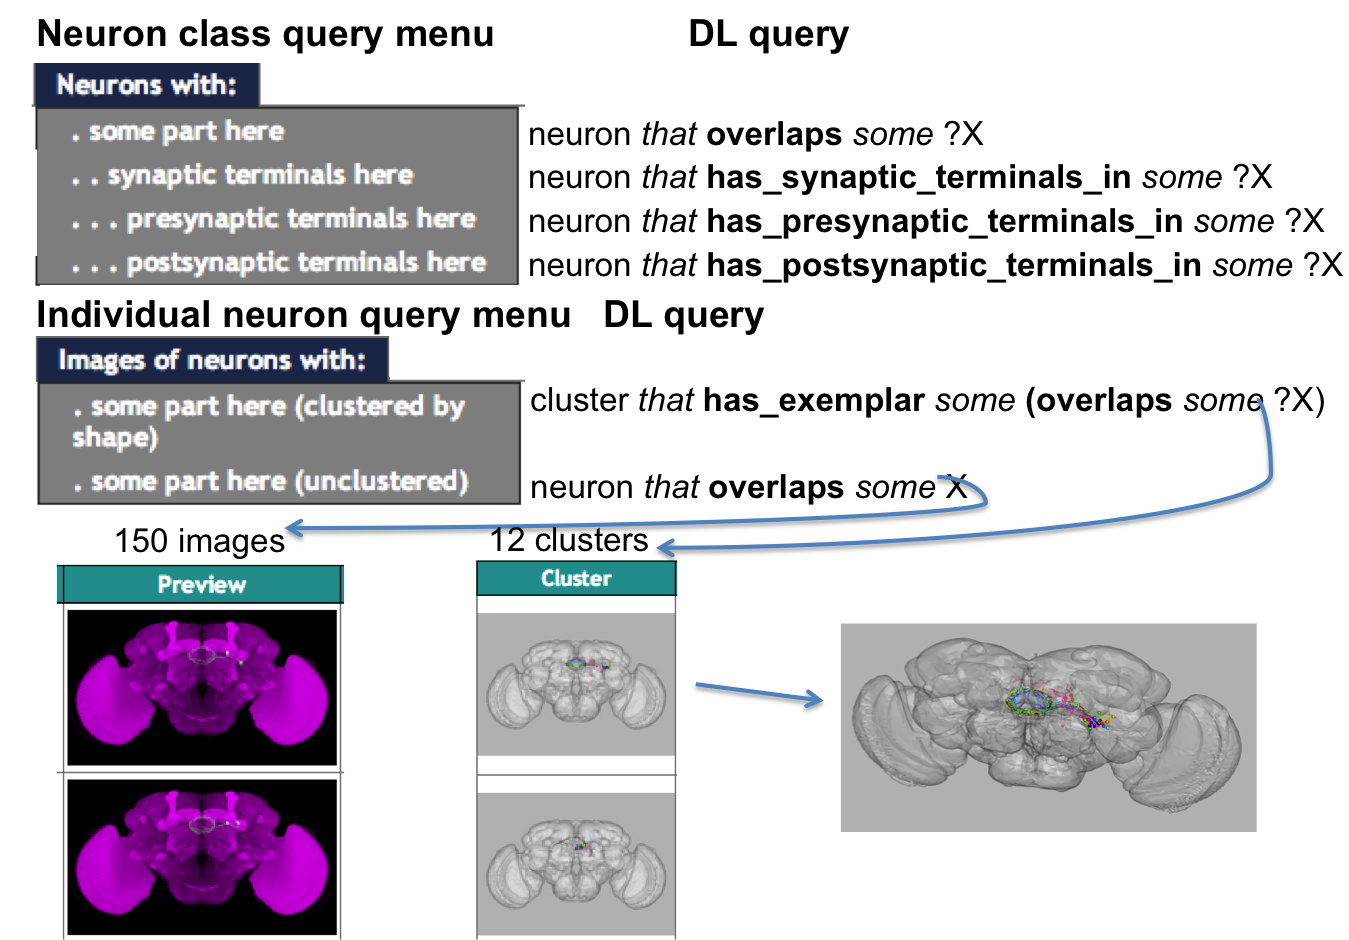
\includegraphics[width=120mm]{images/Query_menus_DL_images.png}
\caption{VFB query menus with the DL queries they run.}
\label{fig:Query_menus_DL_images}
\end{figure}

\section{Integration of images using OWL}

Neurobiology is a very visual subject.  While it is useful to read
both informal and formal descriptions of neuron classes and brain
regions, there is no substitute for being able to see images of them.
VFB is built around a standard, 3D adult brain image.  Major brain
regions are defined as 3D painted regions on this image according to
an expert-defined standard [REF:BrainName].  These regions are modelled as
individual members of the relevant ontology classes, but are also
related to brain region classes via an axiom of the form:

\begin{quote}
\textbf{has\_exemplar} \textit{value} `individual region'
\end{quote}

This indicates that the individual provides a standard reference for
the boundaries of a brain region.  A simple DL query is used to find
images to illustrate term pages for these brain regions.

VFB also incorporates large datasets of 3D images of single neurons
(\textgreater 16,000), neuron clones (\textgreater 200) and expression
patterns (\textgreater 3500). As for painted brain regions, structures
depicted in these images are modelled as OWL individuals.
Importantly, all of these images are registered (morphed) onto the
standard brain. This allows direct comparison - both automated and
manual  - of registered images.

From image analysis, we can determine which gross brain regions a
neuron, clone or expression pattern \textit{overlaps}, recording this
using a \textit{Type} statement on the individual.  These drive queries for
single neuron images by location (figure
\ref{fig:Query_menus_DL_images}). A more sophisticated form of image
analysis, developed by G Jefferis [REF preprint], compares pairs of
neurons,  giving each pair a score for similarity of morphology and
location.  A clustering algorithm is then used to group neurons with
similar morphology and location and to assign an exemplar neuron for
each cluster.

We treat clusters as individuals, with single neurons standing in a
\textbf{member\_of} relationship to a cluster.  A subproperty of
\textbf{member\_of}, \textbf{exemplar\_of}, is used to relate
exemplars to clusters.  This simple formalism allows VFB to group the
very large numbers of images that often result from queries of brain
regions for overlapping neurons into a much smaller number of clusters
of similar neurons (see figure \ref{fig:Query_menus_DL_images}).

In many cases, the resulting clusters correspond largely or completely
to well characterized neurons from the literature, for which the DAO
has classes defined by lineage, tract and location of synaptic
connections. Where this is the case, we add manual typing
statements. In other cases, manual annotation of neurons with
\textit{Type} statements provides sufficient information for automated
classification in the ontology.

\subsection{An owl design pattern for modelling expression patterns}

A key aim of VFB is to provide a means for biologists to find
candidate transgenes suitable for use in genetic dissection of nervous
system function. This is aided immensely by providing images of the
expression patterns found.

We treat expression patterns as anatomical structures defined as the
mereological sum of all cells that express a particular gene or
transgene. We record the expressed gene or transgene shown in all
images, including those of neurons and neuron clones as well as
expression patterns.  But individual neurons and clones are typically
fragments of expression patterns. Users would find it very unintuitive
if queries for expression patterns mixed in images of expression
pattern fragments.   But once an expression pattern has been found,
it is useful to be able to get a list of component parts.

We define \textbf{expresses} using slightly more expressive logic than OWL can
cope with:

\begin{quote}
x \textbf{expresses} y iff:  x \textbf{has\_part} \textit{some} cell \textit{and}
for all cell(c) and \textbf{part\_of} y: (`gene expression'
\textit{and} \textbf{has\_product} \textit{some} y)
\textbf{occurs\_in} c  % Would be better if this were in common logic!
\end{quote}

An expression pattern of a gene/transgene can then be defined and its
partonomy populated using the pattern:

\begin{quote}
`gene B expression pattern'
\textit{EquivalentTo}: `expression pattern' \textit{that} \textbf{expresses} \textit{some} `gene
B'\end{quote}
\begin{quote} \textit{GCI}: \textbf{expresses} \textbf{some} `gene B' \textit{EquivalentTo}
\textbf{part\_of} \textit{some} `B expression pattern'
\end{quote}

% ADD EXAMPLE

This system is currently used on VFB to provide images of transgene
expression patterns found via SQL queries. The above formalisation
provides an obvious way to convert the semi-formalised annotations in
SQL to OWL

For brain regions:

`expression pattern of X' \textbf{overlaps} \textit{some} `brain region Y'

For cells, we can make a stronger assertion:

`expression pattern of X'
\textbf{has\_part}\footnote{\textbf{has\_part} entails \textbf{overlaps}} \textit{some} `cell Y'

We can then find anatomical structures in which there is some
expression via ``\textbf{overlaps} \textit{some} X''

As discussed in the next section, this formalisation can be used to
make safe queries for expression patterns involving negation possible.

%\subsection{An OWL design pattern for modelling lineage clones:}

% Only worth including this if showing useful inference resulting.

%\begin{quote}
%'ALad1 lineage neuron'
%\textit{EquivalentTo}:
%neuron and (\textbf{develops\_from} \textit{some} `neuroblast ALad1')

%\textit{subClassOf}: \textbf{part\_of} \textit{some} `adult ALad1 lineage clone'
%\end{quote}
%


\section{Beyond EL: supporting queries with negation.}

In order to remain computationally tractable and scalable, VFB
restricts expressiveness to the EL profile of OWL and uses the ELK
reasoner \cite{kazakov2012elk} during development and to drive live
OWL queries on the site. Recent advances in reasoning
technology may make scaling with more expressive forms of OWL
practical. For example, Zhou and colleagues have recently published
impressive results for fast query answering by combining triple store
based RL reasoning with a HermiT DL reasoner \cite{ZNCH14a}.

Some types of queries that would be extremely useful to our users
require more expressiveness.  In particular, there are a number of
cases where queries involving negation would be useful.  For example,
for some neurons, we know all of the brain regions overlapped, all of
the tracts fasciculated with and the location of all synaptic
terminals.  It would be useful, in such cases, to allow users to add
negative legs to the compound queries for neuron classes that VFB
already supports.  For some transgene expression
patterns in the adult brain, we have both negative an positive
assertions about where a transgene is expressed.  It would be very
useful for researchers to be able to add negative clauses to queries for
expression as this can be critical to attempts to find sufficiently
specific reagents to use in experiments to genetically dissect the
function of specific neurons and brain regions.

The most efficient way to support queries involving negation is to a
combination of closure axioms and disjointness declarations.  For
example, the neuron DL1 adPN fasciculates with only one tract, the
iACT.  We currently record this as:


\begin{quote}
`DL1 adPN' \textit{subClassOf} \textbf{fascicualtes\_with} \textit{some} iACT
\end{quote}

But if we also have the axioms:

\begin{quote}
`DL1 adPN' \textit{subClassOf} \textbf{fascicualtes\_with} \textit{only} iACT

'great commissure' \textit{disjointWith} iACT
\end{quote}

Then we can find 'DL1 adPN' with the query:
\begin{quote}
	neuron \textit{and not} (\textbf{fascicualtes\_with} \textit{some} `great commissure')
\end{quote}

For cases where a neuron \textbf{fasciculates\_with} multiple tracts, the
closure axioms can simply combine multiple classes using
\textit{or}. Unfortunately, our use of inference over partonomy rules out
this pattern of closure axioms for many important relations used in querying.  For example:

\begin{quote}
\textbf{overlaps} \textit{o} \textbf{part\_of} \textit{subPropertyOf}
\textbf{overlaps}

X \textbf{overlaps} \textit{some} Y

X \textbf{overlaps} \textit{only} Y

Y \textbf{part\_of} \textit{some} Z

Z \textit{disjointWith} X

=\textgreater inconsistency: X \textbf{overlaps} \textit{some} Z, X not (\textbf{overlaps}
\textit{some} Z)
\end{quote}


We can get around this by using closure axioms of the form
``\textbf{rel} \textit{only} (\textbf{has\_part} some X)'' and declaring spatial
disjointness between brain regions (which also provide a useful
integrity check). Spatial disjointness can be declared using a simple
GCI:

\begin{quote}
\textbf{part\_of} \textit{some} X \textit{disjointWith} \textbf{part\_of} \textit{some} Y
\end{quote}

For example, we can represent that the neuron DL1 adPN only has
synaptic terminals in DL1v(part of the antennal lobe) and the lateral
horn\footnote{There is  actually one additional region, but we
  simplify here in order to  provide a more compact example} with:

\begin{quote}
`DL1 adPN'

\textit{subClassOf}: \textbf{has\_synaptic\_terminals\_in}
\textit{some} DL1

\textit{subClassOf}: \textbf{has\_synaptic\_terminals\_in}
\textit{some} `lateral horn'

\textit{subClassOf}: \textbf{has\_synaptic\_terminals\_in}
\textit{only} (\textbf{has\_part} \textit{only} (DL1 \textit{or}
`lateral horn'))

`fan-shaped body' \textit{subClassOf}: \textbf{part\_of} \textit{some}
`central complex'

DL1 \textit{subClassOf}: \textbf{part\_of} \textit{some} `antennal lobe'
\end{quote}

With `antennal lobe', `lateral horn' and  `central complex' declared
spatially disjoint , DL1 adPN is returned by the query:

\begin{quote}
neuron that (\textbf{has\_synaptic\_terminal\_in} \textit{some}
`antennal lobe') and not (\textbf{has\_synaptic\_terminal\_in}
\textit{some} `fan-shaped body')
\end{quote}

An explanation is shown in figure \ref{fig:combined_explanation}B).  There is no need to
assert \textbf{has\_part} relationships. The
\textit{inverseOf} axiom between \textbf{has\_part} and
\textbf{part\_of} is sufficient to infer not \textbf{has\_part} from
spatial disjointness axioms (figure \ref{fig:combined_explanation}A).

This pattern is also dependent on the reflexive nature of
\textbf{part\_of} and \textbf{has\_part} (figure \ref{fig:combined_explanation}B).

\begin{figure}
\centering
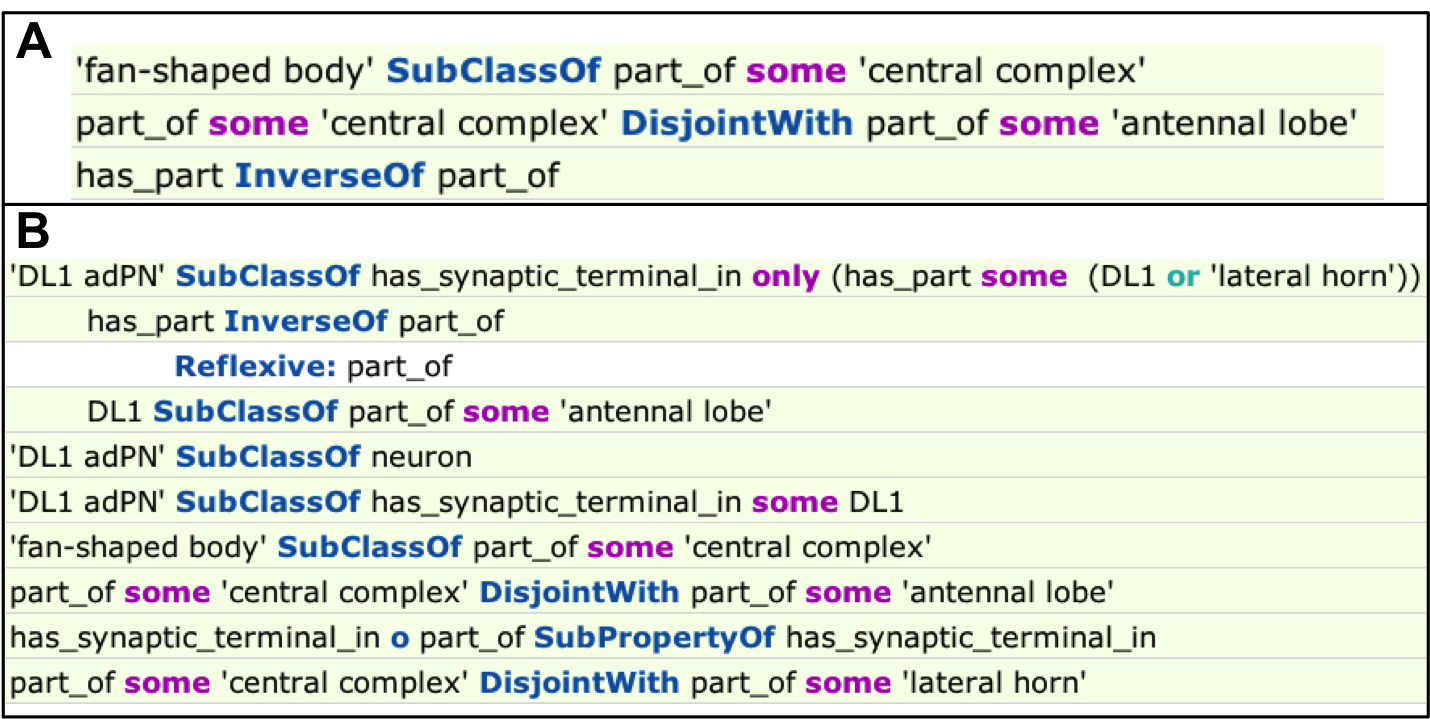
\includegraphics[width=120mm]{images/combined_explanation.png}
\caption{\textbf{A.} Explanation for why the query ``\textit{not}
   \textbf{has\_part} \textit{some} `fan-shaped body' '' returns
   `antennal lobe'.  Note that direct assertion of \textbf{has\_part}
   restriction axioms are not necessary. \textbf{B.} Explanation for
   why the query ``neuron that (\textbf{has\_synaptic\_terminal\_in}
   \textit{some} `antennal lobe') and not
   (\textbf{has\_synaptic\_terminal\_in} \textit{some} `fan-shaped
   body')'' returns the neuron `DL1 adPN'. }
\label{fig:combined_explanation}
\end{figure}

Negative query legs in compound queries for expression patterns would
be especially useful to our users.  Our ability to provide these is
limited by the extent to which it is possible to specify which regions
lack expression.  It is generally not possible to provide an
exhaustive list of all regions that have some part with some level of
expression for a closure axiom with overlaps.  However some datasets
come with explicit assertions about regions not overlapped.  For
example, the largest transgene expression dataset that VFB currently
hosts [Ref Jennett] was provided with annotations recording the
presence or absence of expression in every major neuropil in the adult
brain.  These can easily be translated programmatically into restriction axioms
asserting \textbf{overlaps} and \textit{not} \textbf{overlaps} on
expression pattern classes. % TODO  (fig \cite{fig:} shows an example.)

\section{Discussion and future directions}

% Section summarising VFBs work

Virtual Fly Brain uses OWL to provide a unique service to the
\textit{Drosophila} neurobiology community, integrating a wealth of
information from the literature and bulk datasets into an easily
queryable resource.  Much of this would be difficult or impossible to
provide using a conventional relational database. OWL
provides a sustainable way to develop and maintain a queryable
classification of anatomical structures and neurons.  OWL
axiomatisation allowing inference over partonomy drives queries that
 return complete information about neuronal overlap and synaptic
 terminal location from any level of the partonomy.  OWL reasoning
 also provides a way to group annotations of expression and phenotypes
 based on classification, partonomy and cell overlap.  This massively
 enriches the results of annotation queries.


VFB has so far avoided taking advantage of the full expressiveness of
OWL.  Reasoners such as HermiT and FaCT++ [REFS] are many orders of
magnitude slower at classifying the DAO and answering queries than
ELK, the EL reasoner that we rely on.  They do not even complete when
reasoning across the DAO combined with the VFB knowledgeBase of
individuals.  However, we have one use case for which DL
expressiveness would be extremely useful: compound queries for neurons
or expression patterns involving negation.

There are two major barriers to achieving this. The most serious
barrier is the ability to query across an ontology or combined ontology and
knowledgeBase with DL expressiveness.  Zhou and colleagues have
recently published impressive results for fast query answering by
combining triple store based RL reasoning with a HermiT DL reasoner
\cite{ZNCH14a}.  We are working with the authors to test query speed
for compound queries with negation for test datasets using the design
patterns outlined in this paper.

A more clearly surmountable barrier is the lack of tooling support for
some of the axiomatisation required in the design patterns we propose.  In
particular, adding GCIs to record spatial disjointness is currently
very tedious to do by hand in Protege 5.  This may be achievable by
scripting, but in order for the approach to be accessible for any
ontology builder ideally this would be achievable via a plugin for a
popular editor such as Protege.  By analogy with support for the
addition of class disjointness axioms in Protege, this work by allowing
users to navigate down a partonomy tree, adding disjointness axioms to
whole sets of sibling terms at once.


\section{Methods}

For details of construction and maintenance of the \textit{Drosophila}
anatomy ontology please see Costa et al., 2013 \cite{Costa2013}. The
ontology is available from \url{http://purl.obolibrary.org/obo/fbbt}

VFB is an open source project.  All code is available from
\url{https://github.com/VirtualFlyBrain}
OWL individuals files used on VFB are available from
\url{https://github.com/VirtualFlyBrain/VFB_owl/tree/master/src/owl} % TODO - add
README.md to this page.

A test ontology illustrating implementation of the DL patterns for
negative queries can be found here: TBA!

\subsection{VFB architecture}

All queries for anatomical classes or individuals on VFB are live DL
queries via the elk OWL reasoner.  All queries of annotation begin
with a DL query for subclasses, parts and overlapping cells.  The
resulting list is then used to query annotations store in the FlyBase
Postgresql database.  More details of the overall architecture of the
project cen be found at
\url{https://github.com/VirtualFlyBrain/VFB#overall-architecture-of-project}


\subsection{Database representation of OWL individuals}

Details of individuals are maintained in a SQL database
(\url{https://github.com/VirtualFlyBrain/VFB_owl/wiki/Individuals-DB})
and programmatically converted to OWL via scripting over the OWL-API
(\url{https://github.com/VirtualFlyBrain/VFB_owl/}).  A standard DB
representation of OWL ontologies/individuals would be preferable to
our bespoke solution, which limits axiom expressiveness in order to
keep the DB structure simple.  We are currently unaware of any viable,
non-proprietary alternatives.

\subsection*{Author's contributions}

The OWL design patterns and queries presented in this paper were designed and
tested by DOS  He also designed the database representation of OWL
individuals and wrote the code the translates this representation into
OWL.  The portion of the DAO representing neuroanatomy was built by
DOS and MC.  MC and GJ were responsible for all annotation,
processing and analysis of images. GJ developed the clustering
algorithm and had the idea of assigning exemplars to clusters.

\subsection*{Acknowledgments.}

We thank Simon Reeve for his contributions to the representation of
neuroanatomy in the DAO.  We thank Nestor Milyaev for his work on the
VFB website.

\subsubsection*{Funding}

This work was largely supported by:`Standardising the representation of
Drosophila anatomy and development for databases' ;
BBBSRC:BB/G02233X/1 awarded 2009 to J.Douglas Armstrong, Michael
Ashburner and David Osumi-Sutherland `Structured and graphical queries
for Drosophila neuroscience data'; An Isaac Newton Trust grant to
Cahir O'Kane to fund the work of Marta Costa, Awarded 2012:
`Neuroinformatic identification of new types of neuron in the
Drosophila brain.' VFB is currently supported by a Wellcome Trust
grant to Cahir O'Kane, J. Douglas Armstrong, Gregory S.X.E Jefferis,
Helen Parkinson and David Osumi-Sutherland: `Virtual Fly Brain: a
global informatics hub for Drosophila neurobiology' WT105023MA.


%\begin{thebibliography}{}

\bibliography{../DOS} % Bibliography file (usually '*.bib' )

\bibliographystyle{plain}

%\end{thebibliography}

\end{document}
